\section{\Large{\sffamily{Title}}}

\red This is a template so you don't have to waste time looking up environments for the algorithms, sections, theorems, figures, examples etc.  Please use this template for your essays. The cover page doesn't count for the page limit. \nc

\subsection{Transformation Methods}\label{ssec:transformation}
Given a random variable $X: \Omega \rightarrow E \subseteq \R$, we seek to find a deterministic function $\phi$ such that
$$X=\phi(U),$$
where here and below $U\sim \text{Unif}(0,1)$ and equality is interpreted in distribution. Once such $\phi$ is found, a sample from $f_X$ can be obtained as follows.


\FloatBarrier
\begin{algorithm}
\caption{General transformation method}
\begin{algorithmic}[1]
\STATE {\bf Input}: Transformation $\phi$ such that $X = \phi(U).$
\STATE Set $X^{(n)}=\phi(U^{(n)}),\quad 1\leq n\leq N,$ \quad 
where $U^{(n)}\stackrel{\text{i.i.d.}}{\sim} \text{Unif}(0,1)$.\STATE {\bf Output}: $X^{(n)}\stackrel{\text{i.i.d.}}{\sim}f_X.$
\end{algorithmic}
\end{algorithm}

 


\subsubsection{Inverse Transformation Method}\label{sssec:inversetransformation}
Given a real-valued random variable $X$, the inverse tranformation method is a general way to find $\phi$ with $X = \phi(U).$ It is defined in terms of the CDF $F_X$ of the variable $X.$

\begin{theorem}[Inverse Tranformation Method]\label{thm:inversetransf}
Define $\phi (u):= \inf\{x:F_X(x)\geq u\}\equiv F_X^-(u)$. If $U\sim \emph{Unif}(0,1)$, then $F_X^-(U)=X.$
\end{theorem}
\begin{proof}
We only prove here the case where $F_X$ is a bijection from $(-\infty,\infty)$ to $(0,1).$ In such a case $F_X^-=F_X^{-1}$, see Figure \ref{fig:transformationmethod}.
Then
$$\Prob \bigl(F_X^-(U)\leq x\bigr)=\Prob \bigl(F_X^{-1}(U)\leq x\bigr)=\Prob\bigl(U\leq F_X(x)\bigr)=F_X(x),$$
which shows that the CDF of the random variable $F_X^-(U)$ is $F_X$.
\end{proof}


\begin{remark}
The inverse transform method is simply Algorithm 1 with the choice $\phi (U) : = F_X^-(U)$.
\end{remark}

\noindent
\ \textbf{Advantages of the Inverse Transformation Method}
\vspace{-0.25cm}
\begin{itemize}
\item It is efficient if $F_X^-$ has a closed form expression that can be evaluated cheaply.
\end{itemize}
\noindent
\ \textbf{Disadvantages of the Inverse Transformation Method}
\vspace{-0.25cm}
\begin{itemize}
\item Typically $F_X^-$ does not have a closed form expression that is easy to evaluate.
\vspace{-0.2cm}
\item It is a dead-end: it is not clear how to generalize the method to high dimensional problems where $X$ takes values in $\R^d,$ $d>1,$ even though in some cases it may be possible.
\end{itemize}

  \FloatBarrier
    \begin{figure}[htp]
      \centering
      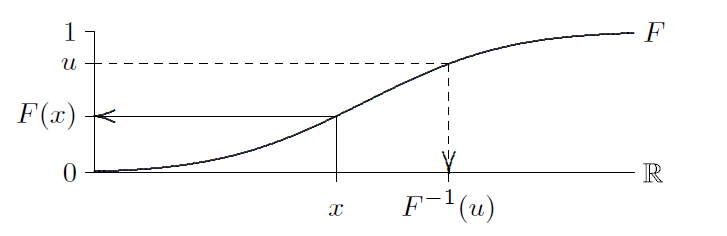
\includegraphics[width=0.75\columnwidth]{transformationmethod.png}
      \caption{A strictly increasing CDF and associated inverse CDF.}
      \label{fig:transformationmethod}
    \end{figure}
    \FloatBarrier



\subsubsection{Other Transformation Methods}\label{sssec:othertransformations}
The inverse transformation method is only one choice of transformation $\phi$ such that $X=\phi(U)$ and in our presentation above is restricted to real-valued variables. Other transformation methods may be applied and their use needs not be restricted to the one-dimensional setting. A classical example is the Box Muller method, which allows to obtain samples $X^{(1)},X^{(2)} \stackrel{\text{i.i.d.}}{\sim} \Nc(0,1)$ (that may be seen as one sample from a bivariate normal dsitribution) from samples $U^{(1)},U^{(2)} \stackrel{\text{i.i.d.}}{\sim} \text{Unif}(0,1)$.

\begin{example}{(Box Muller Method.)} \\
Suppose $X_1,X_2 \stackrel{\text{i.i.d.}}{\sim} \Nc(0,1)$, and write
\begin{align*}
X_1&=R\cos\theta,\\
X_2&=R\sin\theta,\\
\theta &\in [0,2\pi).
\end{align*}
Then blablabla
\end{example}







\subsection{Discussion and Bibliography}

Transformation methods and accept-reject methods can be found in virtually any textbook on Monte Carlo methods, see e.g.  \cite{robert2013monte}. 





